% Preambule
\documentclass[pdftex,french, english]{article}	% the pdftex is essential

% Packages
% ---
\usepackage[utf8]{inputenc}
\usepackage[T1]{fontenc}
\usepackage[dvips]{graphicx}            % to include images
\usepackage{pslatex}	    % to use PostScript fonts
\usepackage{enumitem}
\usepackage{amsfonts}
\usepackage{babel}
\usepackage{algorithm}
\usepackage[noend]{algpseudocode}
\usepackage[paperwidth=17cm, paperheight=22.5cm, bottom=2.5cm, right=2.5cm]{geometry}
\usepackage{csquotes}
\usepackage{multirow}
\usepackage{caption}
\usepackage{hyperref}
\usepackage{tikz}

% modifie les parametres de la balise \paragraph

% where to find images:
\graphicspath{{../images/}}

\setcounter{secnumdepth}{4}
\setcounter{tocdepth}{3}
\makeatletter
\newcounter {subsubsubsection}[subsubsection]
\renewcommand\thesubsubsubsection{\thesubsubsection .\@alph\c@subsubsubsection}
\newcommand\subsubsubsection{\@startsection{subsubsubsection}{4}{\z@}%
                                     {-3.25ex\@plus -1ex \@minus -.2ex}%
                                     {1.5ex \@plus .2ex}%
                                     {\normalfont\normalsize\bfseries}}
\newcommand*\l@subsubsubsection{\@dottedtocline{3}{10.0em}{4.1em}}
\newcommand*{\subsubsubsectionmark}[1]{}
\makeatother

\begin{document}
\selectlanguage{english}

\title{INITIATION A LA RECHERCHE}

\begin{titlepage}
\begin{center}

\textsc{\Large Initiation à la recherche}\\[4em]

\begin{figure}[h]
\begin{center}

\includegraphics{lorraine.png}
\end{center}
\end{figure}

\vspace{4em}
\textsc{\Large \textbf{Planification d'actions \\ dans un monde continu}}\\[3em]
\vspace{4em}
\textsc{\textit{Léopold BELLEC, Pierre-Marie JUNGES}}\\[1em]
\vspace{1em}
\textsc{Encadrants : \textit{Olivier BUFFET, Vincent THOMAS}}\\[1em]


\end{center}

\vspace*{\fill}
\textsc{Master 1 Informatique \hspace*{\fill} 2017}

\end{titlepage}

\newpage
\pagenumbering{arabic}

\selectlanguage{french}
\tableofcontents


\newpage
\selectlanguage{english}
\section{Introduction au problème}
	\subsection{Problématique}
	Une des problématiques importantes en intelligence artificielle est la planification automatique d’actions, que ce soit pour la robotique, pour les jeux (échecs, go, ...), pour la gestion de sources d’énergie, ou pour la protection d’espèces menacées. La plupart des algorithmes développés n’abordent que des situations dans lesquelles le nombre d’états (le nombre de situations) possibles est fini et relativement petit, tout comme le nombre d’actions disponibles. Ces limitations viennent de ce que ces algorithmes raisonnent sur l’arbre des évolutions possible du “système” à contrôler, arbre dont la taille subit une explosion combinatoire avec les nombres d’états et d’actions (et qui n’a plus de sens quand les facteurs de branchement sont infinis).
	\subsection{En quoi ce sujet est-il intéressant ?}

	La principale raison est que les algorithmes que nous allons étudier permettent de résoudre des problèmes proches de l'environnement réel.

	En effet, ces algorithmes peuvent résoudre des problèmes auxquels nous sommes régulièrement confrontés, par exemple, lorsque l'on suit quelqu'un en marchant, inconsciemment nous faisons en sorte que notre vitesse ne soit pas plus rapide (resp. lente) que la personne que nous suivons, nous devons donc accélérer ou réduire notre vitesse.

	Et bien, c'est exactement le genre de problème que ces algorithmes peuvent résoudre.

	De plus, une variante de cet algorithme permettra de gérer des cas où un évènement tiers perturbe les résultats, si nous faisons encore le parallèle avec le monde réel, cet évènement peut être un coup de vent ou bien une glissade.

	C'est pourquoi, nous avons souhaité prendre ce sujet et pousser un peu plus nos connaissances sur les algorithmes de décisions.
	
	\subsection{Notre approche}
	Étant donné le nombre imposant d'états ou d'actions possibles à chaque étape, nous avons donc tout simplement essayer à chaque étape de réduire ce nombre de choix possible jusqu'à avoir un espace plus restreint \cite{couetoux01}.

	C'est donc cette solution que nous avons choisie pour répondre à cette problèmatique. 

	Afin de pouvoir mettre en place l'algorithme, nous avions deux choix d'implémentations, utiliser le langage C ou bien le langage Java. 
	Notre choix s'est finalement porté sur le langage Java, car nous sommes plus habitué à celui-ci et nous trouvons la gestion de mémoire également plus simple.

\section{Le B.A.-BA de l'algorithme MCTS}

	Dans cette partie nous allons introduire les notions importantes relatives à l'algorithme \textbf{M}onte \textbf{C}arlo \textbf{T}ree \textbf{S}earch \cite{coulom01}
	appliqué à un problème discret, c'est-à-dire un problème où le nombre d'états ou actions est fini.

	\subsection{Les bases du Monte Carlo Tree Search}
	\subsubsection{Définition}
	Monte Carlo Tree Search ou bien MCTS est un algorithme de recherche, qui, à partir d'un nœud initial $n_{i}$ indique la meilleure action $a_i$ à utiliser afin d'atteindre un nœud intermédiaire $n_{int}$ proche du nœud terminal recherché $n_{t}$. 

	L'application de méthodes de Monte Carlo fait appel à de nombreuses simulations, cela veut donc dire que lors du déroulement de l'algorithme, un certain nombre d'actions seront joués de manière aléatoire.
	\subsubsection{Déroulement de l'algorithme}
	L'algorithme est exécuté tant que le temps limite $t$ n'est pas écoulé, et se décompose en 4 étapes :
	\begin{figure}[h]
		\centering
		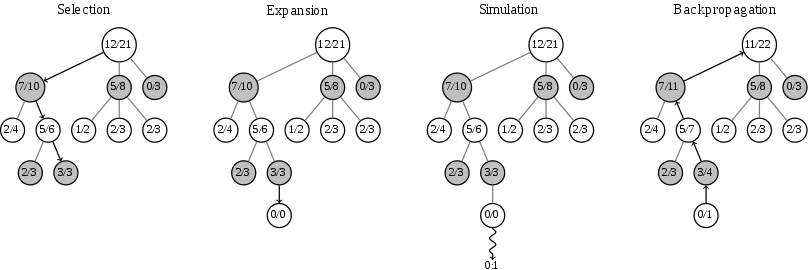
\includegraphics[width=\textwidth]{etapes.png}
		\caption{ Étapes de MCTS}
		 \label{fig:mcts}
	\end{figure}

\textit{Notation : Le nœud correspond à un état du jeu et (12/21) signifie 12 victoires sur 21 simulations.} 
	\begin{enumerate}
		\item \textbf{Sélection}

		À cette étape, l'algorithme va sélectionner parmis ses nœuds suivants le nœud avec la plus grande valeur selon la formule de sélection utilisée \ref{selection}. 

		Dans la figure~\ref{fig:mcts}, on s'aperçoit que l'algorithme sélectionne à tour de rôle le nœud $(7/10)$, puis le nœud $(5/6)$ et enfin le nœud $(3/3)$ et s'arrête car ce nœud n'est pas développé.
		\item \textbf{Expension}

		Une fois le meilleur nœud sélectionné, cette étape va lui rajouter un ou plusieurs nœud(s) enfant, accessible en faisant 1 seule action à partir du nœud courant. 

		Dans la figure~\ref{fig:mcts}, l'algorithme rajoute au nœud courant $(3/3)$ le nœud enfant $(0/0)$.
		\item \textbf{Simulation}

		Maintenant qu'un nouveau nœud a été ajouté, l'algorithme va jouer aléatoirement jusqu'à atteindre un nœud terminal.
		C'est dans cette partie qu'on utilise le principe Monte Carlo, c'est-à-dire l'utilisation de l'aléatoire.
		\item \textbf{Mise à jour} 

		L'algorithme a atteint un nœud terminal, il faut donc récupérer sa récompense (par exemple +1 si c'est un nœud gagnant 0 sinon). Puis faire remonter cette récompense jusqu'au nœud racine et mettre à jour les statistiques de chacun des nœuds parcouru. 

		Dans la figure~\ref{fig:mcts} ci-dessus le nœud terminal était donc perdant car $(0/1)$, donc on va augmenter uniquement le nombre de simulation de chacun de ces nœuds, d'où la transformation du nœud $(3/3)$ en $(3/4)$ par exemple.
	\end{enumerate}
	\subsubsection{Pseudo-code}
	\begin{algorithm}
	\caption{MCTS générique}
	  \label{alg:mcts}
	\begin{algorithmic}[1]
	\Function{MCTS}{État $s$}
	\State création d'un nœud $n$ à partir de $s$
		\While{$temps < tempsLimite $}\Comment{tant qu'il reste du temps}
			\State $n \gets selection(n)$ \Comment{L'étape d'expension est incluse dans cet appel}
			\State $n \gets simulation(n)$
			\State $n \gets miseAjour(n)$
		\EndWhile
	\State \textbf{return} $meilleurEnfant(n)$
	\EndFunction
	\end{algorithmic}
	\end{algorithm}
    
    
	\subsection{Formule de sélection utilisée} \label{selection}
	Précédemment, nous avions parlé lors de l'étape de sélection, de formule de sélection. 
	En effet, afin de choisir le meilleur nœud possible des formules ont été mise en place.


	Et, c'est dans cette partie que nous allons en expliquer une (la principale utilisée), puis de nouvelles seront introduites
	dans la section suivante \ref{continu}.

	\textit{Notation : Soit $n$ un nœud, $N$ son nœud parent, et C une constante d'exploration.} 

	\begin{enumerate}
		\item Upper Confidence Bounds (\textbf{UCB}) \\
		\[ \frac{recompenses(n)}{simulations(n)} + C \times \sqrt{\frac{simulations(N)}{simulations(n)}} \] 

		On se rend compte ici que si notre constante d'exploration \textit{C} est égale à $0$ alors, l'algorithme va choisir le nœud $n$ avec le meilleur rapport $\frac{recompenses(n)}{simulations(n)}$ possible. 

		Donc si l'on souhaite permettre l'exploration de l'arbre, il faut que la constante $C$ soit différente de $0$ sinon on voit bien qu'à l'état initial l'algorithme sélectionne un nœud $n$, alors ce dernier aura nécessaire le meilleur rapport $\frac{recompenses(n)}{simulations(n)}$ vu qu'il est le seul à avoir été développé et,  il sera tout au long de l'algorithme choisit. 


		\underline{\textbf{Lexique}} : On utilise le terme UCT (\textit{Upper Confidence Bound for Trees}) pour désigner l'algorithme MCTS utilisant une formule de sélection de type UCB.
	\end{enumerate}





	\subsection{Stratégies de sélection terminale}
	Les formules explicitées ci-dessus ont pour rôle de choisir le meilleur enfant lorsque l'algorithme se trouve à l'étape de sélection. 

	Dans cette partie, l'algorithme est terminé et l'arbre a été développé. Nous ne pouvons donc plus réutiliser les formules précèdentes car la constante d'exploration \textit{C} n'a plus de sens ici. 

Il faut donc trouver d'autres moyens pour choisir le meilleur nœud enfant. 
Cette étape correspond à l'appel \textit{meilleurEnfant(n)} dans l'algorithme~\ref{alg:mcts}. 
Or, nous savons qu'un nœud $n$ possède un nombre de simulation, et de récompense.
	À partir de ces deux informations nous avons utilisé 3 stratégies de sélection :
	\begin{enumerate}
		\item Robuste :
		
		On choisit le nœud avec le plus grand nombre de simulation.
		\item Maxi :  
		
		On choisit le nœud qui possède la valeur de récompense la plus élevée.
		\item Maxi-Robuste :
		
		On choisit le nœud ayant le meilleur rapport $\frac{recompense}{simulation}$.
	\end{enumerate}
    
    
    
    
    
	\subsection{Application sur un exemple}
	Maintenant que nous avons vu comment l'algorithme fonctionnait de manière générale, nous l'avons mis en pratique sur le jeu du type Puissance $4$. 
    

    Pour rappel voici la règle du jeu selon wikipedia\footnote{\url{https://fr.wikipedia.org/wiki/Puissance_4}} :
   
    \begin{displayquote}
    \textit{``Le but du jeu est d'aligner 4 pions sur une grille comptant 6 rangées et 7 colonnes. Chaque joueur dispose de 21 pions d'une couleur (par convention, en général jaune ou rouge). Tour à tour les deux joueurs placent un pion dans la colonne de leur choix, le pion coulisse alors jusqu'à la position la plus basse possible dans la dite colonne à la suite de quoi c'est à l'adversaire de jouer. Le vainqueur est le joueur qui réalise le premier un alignement (horizontal, vertical ou diagonal) d'au moins quatre pions de sa couleur. Si, alors que toutes les cases de la grille de jeu sont remplies, aucun des deux joueurs n'a réalisé un tel alignement, la partie est déclarée nulle.''}
   	\end{displayquote}


	Après de nombreux essais, humain contre ordinateur, nous avons remarqué qu'il était très compliqué voir impossible de battre l'algorithme à partir d'un certain temps $t$, et sur un ordinateur avec un processeur type $i7$ ce temps est d'environ $2$ secondes.
	

Afin de poursuivre un peu plus notre expérience, nous avons décidé de faire jouer $2$ ordinateurs l'un contre l'autre, et, de cette facon, comparer les différentes stratégies de sélection finales et voir si effectivement certaines sont plus efficaces que d'autres.
		\\
		\begin{table}[h]
		\begin{tabular}{cc|c|c|c|c}
			\cline{3-5}
			& & \multicolumn{3}{ c| }{Ordinateur 2} \\ \cline{3-5}
			& & Robuste & Maxi & Robuste-Maxi \\ \cline{1-5}
			\multicolumn{1}{ |c  }{\multirow{3}{*}{Ordinateur 1} } &
			\multicolumn{1}{ |c| }{Robuste} & 70-30-0 & 60-40-0 & 60-40-0 &    \\ \cline{2-5}
			\multicolumn{1}{ |c  }{}                        &
			\multicolumn{1}{ |c| }{Maxi} & 80-20-0 & 80-20-0 & 50-50-0 &     \\ \cline{2-5}
			\multicolumn{1}{ |c  }{}                        &
			\multicolumn{1}{ |c| }{Maxi-Robuste} & 90-10-0 & 60-40-0 & 70-30-0 &     \\ \cline{1-5}
		\end{tabular}
			\caption{Comparatif des différentes stratégies}\label{tabular:compa}
		\end{table}

\underline{\textit{Méthodes expérimentales et explications de la table~\ref{tabular:compa}}} : 
\\ \\
L'ordinateur 1 commence \textbf{toujours} les parties, la notation $x-y-z$ signifie $x\%$ de victoire(s) pour l'ordinateur 1, $y\%$ de victoire(s) pour l'ordinateur 2, $z\%$ de match(s) nul(s).

Comme nous pouvons le remarquer, l'ordinateur commencant la partie à globalement plus de chance de gagner, peu importe la stratégie utilisée.


Réfléchissons sur la stratégie Maxi, dans le jeu Puissance $4$ nous avons fixé la récompense en cas de victoire à $1$ peu importe si la victoire était "serrée" ou bien "écrasante". 

Or plaçons nous maintenant dans le cas où nous aurions fait des récompenses différentes selon le type de victoire, posons par exemple $1$ par une victoire "serrée" et $10$ pour une victoire "écrasante". 

De ce fait, si nous avions un nœud avec $19$ de récompense décomposé en $19$ victoires dites "serrées" et $1$ défaite, et un autre nœud avec $20$ de récompense mais composée seulement de $2$ victoires "écrantes" et $18$ défaites.
Alors dans ce cas, la stratégie Maxi nous retournera le nœud avec $20$ de récompense alors que nous aurions pu prendre le nœud qui a $19$ victoires sur $20$ simulations et qui est donc plus intéressant car son pourcentage de victoire est plus élévé.

Donc, pour pouvoir utiliser la stratégie Maxi de manière efficace, il est préférable de l'utiliser sur un jeu où l'on a une unique récompense en cas de victoire (ce qui est le cas ici).
\\ \\
Utilisons maintenant ce même raisonnement ainsi que ce même cas de figure pour la stratégie Robuste, nous avons donc $2$ nœuds avec $20$ simulations chacuns. 

Or on est censé choisir le nœud ayant le maximum de simulations possible, donc notre stratégie Robuste va tout simplement retourner le premier nœud lu car le deuxième nœud lu n'aura pas un nombre de simulation strictement supérieur au premier nœud. Alors, dans notre cas de figure, la stratégie Robuste aura une probabilité de $\frac{1}{2}$ de retourner le meilleur nœud (celui avec les $19$ victoires).

Donc, de la même façon que la stratégie Maxi, la stratégie Robuste n'est pas nécessairement bonne pour choisir le meilleur nœud possible.
\\ \\
À partir des raisonnements ci-dessus il est donc facile de se convaincre que choisir la stratégie Maxi-Robuste est préférable, car le fait qu'elle prenne le meilleur rapport $\frac{recompense}{simulation}$ l'empêche donc d'être biaisé, car son choix dépend de 2 critères différents.

\newpage

\section{Application dans un monde continu} \label{continu}

Maintenant, que nous avons vu comment fonctionne le MCTS dans un monde discret, dans cette partie nous étudierons son fonctionnement dans un monde continu à travers 3 variantes différentes.
	\subsection{Définition}

	À la différence d'une variable discrète, qui a donc un ensemble de valeurs possibles fini; une variable continue est une variable dont l'ensemble des valeurs possibles est infini.

	Par un exemple : supposons que nous avons une voiture, sa vitesse correspond donc à une variable continue car elle peut être de $40,00$ km/h tout comme de $16,24575$ km/h, il existe donc une infinitée de valeurs réelles entre les intervalles $0$ km/h et $Vitesse_{max}$ km/h. \\

	Donc, dans cette partie, nos différentes variantes de MCTS vont travailler avec des variables de ce type.

	\subsection{Explications du problème}

	Voici une illustration du problème \cite{couetoux01} que nous allons essayer de résoudre : \\

	\begin{figure}[h]
	\centering
		\begin{tikzpicture}
		% axe abscisse
		\draw[->] (1, 1) node[below] {0} -- (5, 1) node[below] {position};

		% axe ordonné
		\draw[->] (1, 1) -- (1, 5) node[right] {récompense};

		% premier palier
		\draw (1, 2) -- (2, 2);
		\draw (2, 1) -- (2, 2);

		% deuxieme palier
		\draw (2.7, 1) -- (2.7, 3);
		\draw (2.7, 3) -- (5, 3);

		% double fleche a
		\draw[<->] (0.75, 1) -- (0.75, 2) node[pos=.5, left] {a = 70};

		% double fleche l
		\draw[<->] (1, 2.25) -- (2, 2.25) node[pos=.5, above] {l = 1};

		% double fleche w
		\draw[<->] (2, 0.75) -- (2.7, 0.75) node[pos=.5, below] {w = 0.7};

		% double fleche h
		\draw[<->] (5.25, 1) -- (5.25, 3) node[pos=.5, right] {h = 100};

		\end{tikzpicture}
		\caption{Illustration du problème} \label{fig:probleme}
	\end{figure}

	Notre algorithme va partir de la position initiale $0$, puis devra en $2$ actions, maximiser les récompenses cumulées.

	Pour ce faire la fonction récompense est définie ainsi :
	$$recompense(x) = \left\{
	\begin{array}{ll}
 	a & \mbox{ si $x <= l$}\\
 	0 & \mbox{ si $l < x < l + w$}\\
 	h & \mbox{ si $x >= l + w$}
 	\end{array}\right.$$

	Sachant qu'une action $\in [0, 1]$, et que la récompense cumulée optimale est de $170$ (décomposée en $70 + 100$).
	La principale difficultée ici réside dans le fait qu'il existe un "piège" illustré par la variable $w$ située entre les positions $1$ et $1.7$.

	Il va donc être intéressant de voir si l'algorithme préfère effectuer $2$ actions dans l'intervalle $[0,1]$ et donc obtenir en récompenses cumulées
	$140$ ou bien s'il va essayer de franchir ce fameux piège et ainsi obtenir la récompense optimale.

	\subsection{Première approche}
		\subsubsection{Modification du MCTS discret}

		Étant donné que nous avions passé quelques temps sur le MCTS discret, nous avons essayé de ré-utiliser ce dernier.

		Cependant, nous avons donc été confronté à une première problématique : "Comment faire fonctionner un problème ayant des variables continues dans un algorithme fait pour des problèmes discrets ?" \\

		Et la réponse est simple, nous avons tout bonnement créé une entité permettant de faire la jonction entre le problème continu et notre MCTS discret. 

		Et ce type d'entité, en programmation logicielle, correspond à un design pattern $Adapter$.\\

		Ci-dessous un diagramme de séquence simplifié ~\ref{fig:actionsPossibles}, pour mieux comprendre, ce que donne ce système lorsque le MCTS va demander à un problème ses actions possibles.
		\begin{figure}[H]
			\centering
			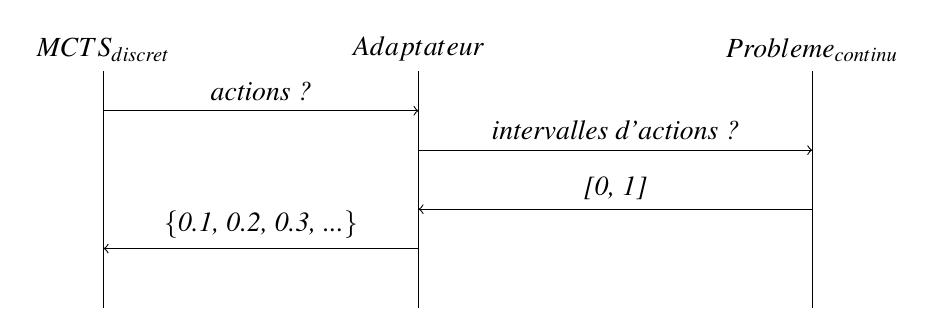
\begin{tikzpicture}
				% axe MCTS discret
				\draw (1, 2) -- (1, 5) node[above] {$MCTS_{discret}$};

				% axe adaptateur
				\draw (5, 2) -- (5, 5) node[above] {$Adaptateur$};

				% axe simulateur
				\draw (10, 2) -- (10, 5) node[above] {$Probleme_{continu}$};

				% segment actions ?
				\draw[->] (1, 4.5) -- (5, 4.5) node[pos=.5, above] { \textit{actions ?} };

				% segment intervalle d'actions ?
				\draw[->] (5, 4) -- (10, 4) node[pos=.5, above] { \textit{intervalles d'actions ?} };

				% segment réponse intervalle probleme->adaptateur
				\draw[->] (10, 3.25) -- (5, 3.25) node[pos=.5, above] { \textit{[0, 1]} };

				% segment réponse intervalle adaptateur->mcts
				\draw[->] (5, 2.75) -- (1, 2.75) node[pos=.5, above] { \textit{\{0.1, 0.2, 0.3, ...\}} };
			\end{tikzpicture}
			\caption{Obtenir les actions possibles d'un problème continu dans le MCTS discret} \label{fig:actionsPossibles}
		\end{figure}

		Néanmoins, nous verrons dans la partie \ref{exp:mctsD} que cette modification n'est pas aussi efficace que les deux prochains algorithmes.
	\subsection{Progressive widening} \label{pw}

		\subsubsection{Principe} \label{pw:principe}

		Contrairement à la version précédente, cette amélioration permet de résoudre des problèmes dont le nombre d'actions est très grand voire infini sans utiliser d'adaptateurs ou autres artifices.

		De plus, cet algorithme garde à peu près la même structure que l'algorithme générique MCTS \ref{alg:mcts}, la principale différence est que les étapes $selection(n)$ et $simulation(n)$ seront regroupées en une seule étape.

		Étant donné le fait que nous avons pour tout nœud $n$ un nombre extrêmement grand d'actions possibles, cet algorithme va donc à chaque itération ajouter (ou non) à la liste des actions possibles d'un nœud courant, une ou plusieurs action(s) supplémentaire(s).

		Afin de savoir si l'algorithme doit ajouter une ou plusieur(s) action(s), on va principalement utiliser le nombre de simulation, noté $t$, du nœud courant.
		Puis le principe sera le suivant : initialemment, un nœud aura une liste d'actions possibles de taille égale à la valeur de la constante d'exploration $C$ \ref{selection} utilisée, puis plus le nœud sera visité plus sa liste d'actions possibles augmentera.

		Ce principe nous permet de développer de manière efficace les nœuds les plus visités, donc les nœuds plus intéressants.

		\subsubsection{Pseudo-code} \label{pw:code}

		\begin{algorithm}[H]
			\caption{Progressive widening (PW) appliqué à un État $s$ avec la constante d'exploration $C > 0$ and $\alpha \in ]0, 1[$.}
			\label{alg:spw}
				\begin{algorithmic}[1]
					\Function{PW}{État $s$}
						\State $nbSimulation(s) \gets nbSimulation(s) + 1$ 
						\State $t \gets nbSimulation(s)$
						\State $k \gets \lceil{C \times t^{\alpha}}\rceil$
						\State \textit{// On va parcourir les actions possibles entre 0 et k}
						\For{$i \in [0 ,k]$}
							\State \textit{/* On récupère la récompense de s plus la récompense si on applique $action_{i}$ à $s$ */}
							\State $recompense \gets recompense(s) + recompense(s, action_{i})$
							\State \textit{// On récupère le nombre de simulation où $action_{i}$ a été appliqué à $s$}
							\State $nb \gets nbSimulation(s, action_{i})$
							\If{$nb = 0$}
								\State \textit{/* Si $action_{i}$ fournit un État jamais exploré, alors on retourne ce dernier */}
								\State \textbf{return} $(s, action_{i})$
							\Else
								\State \textit{// Sinon on calcul le score correspondant}
								\State $score(i) \gets \frac{recompense}{nb} + \textbf{$k_{ucb}$}\sqrt{\log(t)/(nb + 1)}$							
							\EndIf
						\EndFor
						\State \textit{// La boucle for est terminée, on recupère l'indice ayant le score maximal}
						\State $i_{max} \gets indiceMaximisant(score)$
						\State \textbf{return} $(s, action_{i_{max}})$
					\EndFunction
				\end{algorithmic}
		\end{algorithm}

		Même si nous avions explicité dans la partie \ref{pw:principe} quelle était la différence entre le MCTS générique \ref{alg:mcts} et le MCTS avec le progressive widening, voici tout de même le pseudo code de ce dernier \ref{alg:mctspw}.

		\begin{algorithm}[H]
			\caption{MCTS avec le progressive widening}
			\label{alg:mctspw}
				\begin{algorithmic}[1]
					\Function{MCTS}{État $s$}
						\While{$temps < tempsLimite $}\Comment{tant qu'il reste du temps}
							\While{$s$ n'est pas terminal}
								\State $s \gets PW(s)$ \Comment{On applique le progressive widening à $s$}
							\EndWhile
						\State $s \gets miseAjour(s)$
						\EndWhile
						\State \textit{/* Lorsque le temps est écoulé, on applique la stratégie robuste pour déterminer le meilleur prochain État */}
					\State \textbf{return} Robuste($s$)
					\EndFunction
				\end{algorithmic}
		\end{algorithm}
	\subsection{Double progressive widening} \label{dpw}
		\subsubsection{Principe} \label{dpw:principe}

			Cette seconde amélioration prend la même base que le progressive widening \ref{pw} mais permet, en plus de gérer un nombre d'action très grand, gérer le cas où, lorsque l'on a sélectionné la meilleure action possible, un bruit parasite se produit.

			De ce fait, en un seul appel, la fonction double progressive widening va produire à partir d'un état $s$ (potentiellement) 2 nœuds (pas de 2 fils).

			Le premier nœud fils, noté $s'$ correspondra à la meilleure action $a$ appliqué à l'état $s$ (même principe que PW); puis le second nœud noté $s''$, un nœud fils du premier nœud, correspondra à un bruit parasite appliqué à $s'$.
			Dans notre cas, le bruit est toujours additif, néanmoins l'algorithme est censé marcher peu importe si le bruit est additif ou soustractif.

			Afin de savoir si l'on doit ajouter un bruit, le double progressive widening va principalement utiliser le nombre de simulation ainsi que le nombre d'enfants de l'état $s'$.

			Puis le principe sera le suivant: plus un état $s'$ sera simulé, plus il aura de chance d'être bruité, donc d'avoir un nouvel enfant $s''$. Néanmoins, à partir d'un certain seuil aucun enfant ne sera ajouté, et l'algorithme retournera alors un enfant tiré aléatoirement parmi les enfants de $s'$.

			Donc, cet algorithme va nous permettre de gérer des situations dans lesquelles un évènement tiers perturbe les résultats, type d'évènement que l'on retrouve très souvent dans la vie de tous les jours. Par exemple, en hiver avec les plaques de verglas, pour calculer les pas optimaux à faire afin de ne pas tomber où glisser 

		\subsubsection{Pseudo-code} \label{dpw:code}

			\begin{algorithm}[H]
				\centering
				\caption{Double progressive widening (PW) appliqué à un État $s$ avec la constante d'exploration $C > 0$ and $\alpha \in ]0, 1[$.}
				\label{alg:dpw}
					\begin{algorithmic}[1]
						\Function{DPW}{État $s$}
							\State $nbSimulation(s) \gets nbSimulation(s) + 1$ 
							\State $t \gets nbSimulation(s)$
							\State $k \gets \lceil{C \times t^{\alpha}}\rceil$
							\State \textit{// On va parcourir les actions possibles entre 0 et k}
							\For{$i \in [0 ,k]$}
								\State \textit{/* On récupère la récompense de s plus la récompense si on applique $action_{i}$ à $s$ */}
								\State $recompense \gets recompense(s) + recompense(s, action_{i})$
								\State \textit{// On récupère le nombre de simulation où $action_{i}$ a été appliqué à $s$}
								\State $nb \gets nbSimulation(s, action_{i})$
								\If{$nb = 0$}
									\State \textit{// Si $action_{i}$ renvoit un état jamais exploré, alors on retourne cet état}
									\State \textbf{return} $(s, action_{i})$
								\Else
									\State \textit{// Sinon on calcul le score correspondant}
									\State $score(i) \gets \frac{recompense}{nb} + \textbf{$k_{ucb}$}\sqrt{\log(t)/(nb + 1)}$							
								\EndIf
							\EndFor
							\State \textit{// La boucle for est terminée, on recupère l'indice ayant le score maximal}
							\State $i_{max} \gets indiceMaximisant(score)$
							\State $s' \gets (s, action_{i_{max}})$ \Comment{On récupère le meilleur enfant dans s'}
							\State $nb \gets nbSimulation(s')$
							\State $nbEnfant \gets nbEnfant(s')$
							\State $k' \gets \lceil{C \times nb^{\alpha}}\rceil$
							\If{$k' > nbEnfant$}
								\State $s'' \gets bruitage(s')$ \Comment{On applique un bruit à s'}
								\If{$s'' \notin enfants(s')$}
									\State $enfants(s') \gets enfants(s') \cup s''$ \Comment{On ajoute s'' comme enfant de s'}
									\State \textbf{return} $s''$ \Comment{On retourne l'enfant bruité}
								\Else
									\State \textbf{return} $s''$ \Comment{On retourne l'enfant bruité}
								\EndIf
							\Else
								\State \textit{// Sinon on retourne un enfant tiré aléatoirement dans s'}
								\State \textbf{return} $enfantAleatoire(s')$
							\EndIf
						\EndFunction
					\end{algorithmic}
			\end{algorithm}
			
			\newpage
			Et voici, l'algorithme MCTS avec la stratégie double progressive widening \ref{alg:mctsdpw}, cet algorithme reste structurellement très proche de l'algorithme MCTS avec progressive widening \ref{alg:mctspw}
			\begin{algorithm}[H]
			\centering
			\caption{MCTS avec le double progressive widening}
			\label{alg:mctsdpw}
				\begin{algorithmic}[1]
					\Function{MCTS}{État $s$}
						\While{$temps < tempsLimite $}\Comment{tant qu'il reste du temps}
							\While{$s$ n'est pas terminal}
								\State $s \gets DPW(s)$ \Comment{On applique le double progressive widening à $s$}
							\EndWhile
						\State $s \gets miseAjour(s)$
						\EndWhile
						\State \textit{/* Lorsque le temps est écoulé, on applique la stratégie robuste pour déterminer le meilleur prochain État */}
					\State \textbf{return} Robuste($s$)
					\EndFunction
				\end{algorithmic}
		\end{algorithm}
\subsection{Expérimentations} \label{exp}
	\subsubsection{MCTS discret dans un monde continu} \label{exp:mctsD}
	\subsubsection{Progressive widening} \label{exp:pw}
			\subsubsubsection{Sans ajout de bruit}
		\subsubsubsection{Avec ajout de bruit}
	\subsubsection{Double progressive widening} \label{exp:dpw}
\subsection{Conclusion}
\newpage
\selectlanguage{french}
\bibliographystyle{alpha}
\bibliography{biblio.bib}

\end{document}